
\chapter{IPv6 op globaal niveau}
\label{ch:h5}

In dit hoofdstuk zal er dieper worden ingegaan op de adoptie van IPv6 op verschillende niveaus. Er zal bekeken worden hoe deze overgang loopt op zowel globaal niveau als een klein deel op Europees en Belgisch niveau. Dit zou een goede schets moeten geven over hoe het er in België momenteel aan toe gaat en of we al dan niet een betere verhouding hebben dan andere landen. 

\section{Hoe staat IPv6 er tegenover}

Het is ook al eerder geweten dan vandaag dat de uitputting van IPv4 tot zijn einde is gekomen. De beschikbare adressen zijn bijna volledig uitgedeeld en het einde is nabij. Als gevolg hiervan was er IPv6 ontwikkeld om IPv4 over te nemen na zijn uitputting. Dankzij de ‘World IPv6 Day’ is de groei en het aantal gebruikers van IPv6 zeker gestegen. Vanaf deze dag is IPv6 officieel aangekondigd als opvolger van IPv4. 

\section{IPv6 op globaal niveau}

IPv6 is wereldwijd bekend, het nieuwe internet protocol. Hier zal er verder onderzocht worden wat de huidige status is over het internationale gebruik van IPv6. Hoe bedrijven, landen en gebruikers zich hieraan gaan aanpassen en of dit wel effectief bekend is en gebruikt wordt. Het globaal bekijken van het gebruik van IPv6 kan op verschillende manieren gebeuren. Er zal gebruik gemaakt worden van grafieken die geanalyseerde data grafisch zal voorstellen. Verschillende grafieken zullen vergelijkingen weergeven op verschillende aspecten die onderzocht kunnen worden. Alsook het analyseren van globale enquêtes. 

Een eerste grafiek zal aantonen hoeveel gebruikers er zijn, die Google bereiken over IPv6. Deze grafiek geeft een duidelijke weergave van de groei die afgelopen jaren volgde en vooral vanaf 2011, de dag waarop IPv6, begon met evolueren. De laatste meting was op 22 mei 2018 en bevatte een totaal van 19.25\% IPv6 gebruikers. Dit wilt verder zeggen dat bijna 1 op de 5 personen Google bereikt via IPv6. 

\begin{figure}
\centering
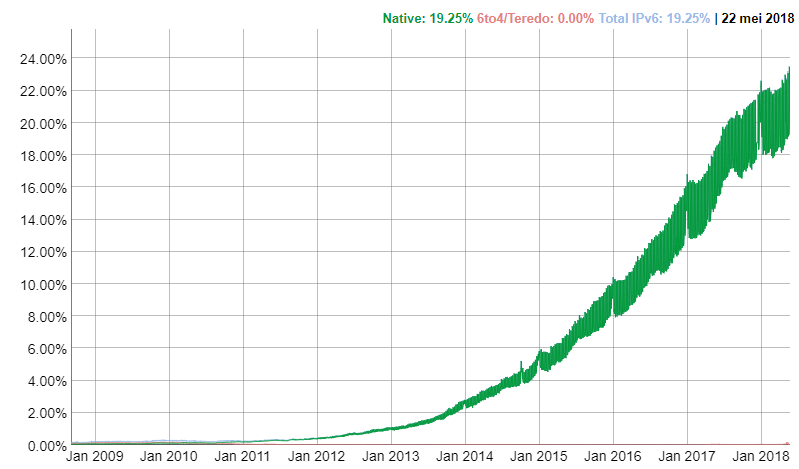
\includegraphics[width=\textwidth,height=\textheight,keepaspectratio]{googleIPv6.png}
\caption{IPv6 evolutie van Google \autocite{GoogleIPv6}}
\end{figure}

Een volgende grafiek geeft weer hoeveel /48 blokken er uitgedeeld zijn van IPv6. Als we deze grafiek dieper gaan onderzoeken, zijn er twee stijgingen te zien. De eerste stijging vond plaats vanaf 2004 tot en met 2006. Deze evolutie is vooral te danken aan de eerste opkomst van IPv6. De tweede groei, waarbij deze nog niet is gestopt en dus nog steeds aan het doorgroeien is, is begonnen in 2011. Hier kunnen we zeggen dat dit gekomen is door de dag van IPv6 dat was uitgeroepen in 2011. Ook is er te zien dat vanaf het jaar 2011 een blijvende stijging is wat het zeer goed maakt voor de populatiegroei van IPv6. De laatste meting, op 1 mei 2018, telt 15.281.735.778 /48 blokken wereldwijd. 

\begin{figure}
\centering
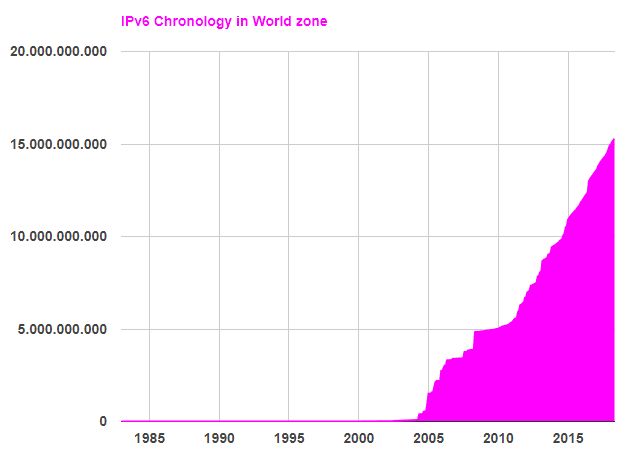
\includegraphics[width=\textwidth,height=\textheight,keepaspectratio]{48blokIPv6.PNG}
\caption{IPv6 /48 blok visueel \autocite{RIR2018}}
\end{figure}

Onderstaande grafiek geeft ons een breder beeld over het percentage netwerken, autonome systemen, dat een IPv6 prefix aankondigd. Globaal gezien is er een gemiddelde van 24.37\%, waarvan 14738 van de 60473 Ases, IPv6 geactiveerde netwerken. Deze laatste meting werd genomen op 1 maart 2018.

\begin{figure}
\centering
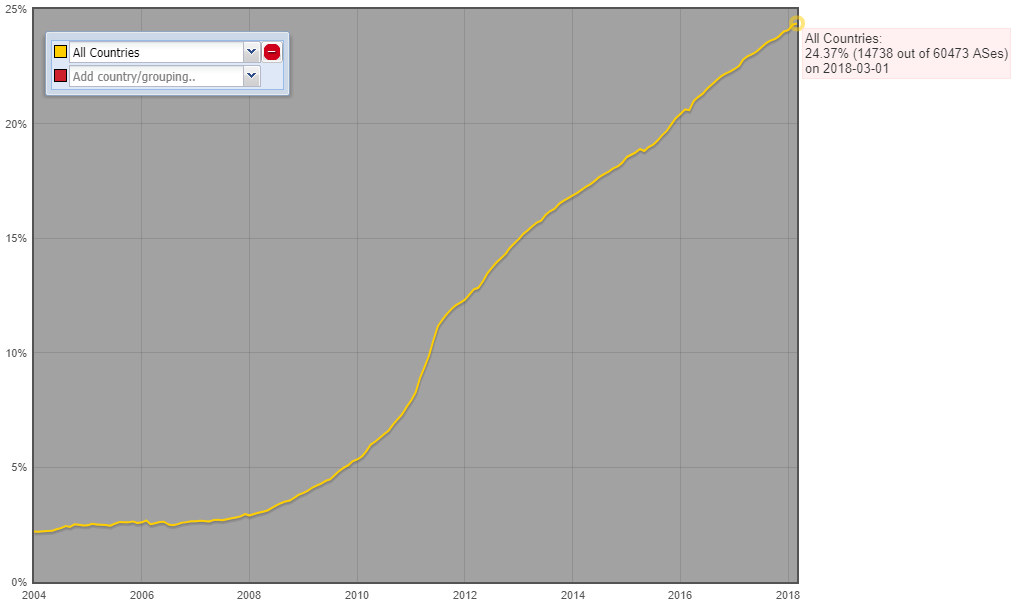
\includegraphics[width=\textwidth,height=\textheight,keepaspectratio]{asIPv6.PNG}
\caption{IPv6 autonome systemen \autocite{RIPE2016}}
\end{figure}

Er is ook een duidelijk overzicht van welk land het beste scoort op verschillende onderdelen van IPv6 gebruik. Dit gebruik kan onderverdeeld worden in 4 verschillende categorieën namelijk, Web, Email, DNS en IPv6 actieve gebruikers.

Vervolgens heeft RIPE enkele enquêtes opgesteld om te meten wat de ondervindingen zijn en hoe het zit met het uitrollen van IPv6. Hiermee kan er onderzocht worden hoe de aanpak, adoptie en aanvaardingen zijn van IPv6. Verder gaan er enkele enquêtes aangekaart worden en met elkaar vergeleken worden. Deze zullen een duidelijk overzicht geven van de overgang van IPv6 op jaarniveau. Hiermee kan er onderzocht worden hoe groot de evolutie is op de voorbije jaren.

De eerste enquête die werd opgesteld dateert van 14 November 2016, de intentie hiermee was om een breder beeld te creëren over de huidige uitrolling van IPv6 was, specifiek gericht op ISP’s. 

De eerste grafiek geeft een zeer informatief beeld terug. Hierop is beter te zien dat de respons op de enquête uit twee soorten gebruikers bestaat. De eerste groep heeft IPv4 gebruikt, de andere groep gebruikte IPv6 om deze enquête te beantwoorden. Dit geeft ons dus al een beter beeld van hoeveel percent van de gebruikers het IPv6 protocol hanteren. In 2016 was dit maar liefst 31\%, 372 van de 1199 deelnemers, hebben over IPv6 beantwoord. 

\begin{figure}
\centering
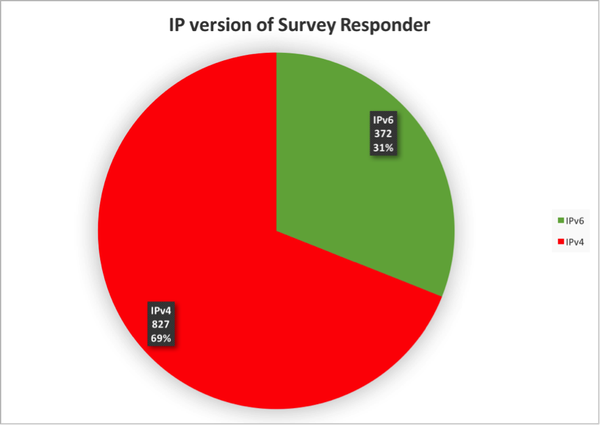
\includegraphics[width=\textwidth,height=\textheight,keepaspectratio]{survey2016_aantal.png}
\caption{IPv6 survey 2016 respons \autocite{Martinez2016}}
\end{figure}

Een volgende grafiek geeft beter aan van waar deze deelnemers komen en onder welke instantie ze vallen. Met instanties wordt er bedoeld onder welke regio de deelnemers vallen. Op onderstaande grafiek is er dus duidelijk te zien dat de meeste uit de regio RIPE NCC komen. Deze instantie is verantwoordelijk voor de Europese kant. Waaronder ARIN verantwoordelijke is voor de Amerikaanse regio, AfriNIC voor de Afrikaanse, APNIC voor de Aziatische en de LACNIC voor de Latijns-Amerikaanse regio.

\begin{figure}
\centering
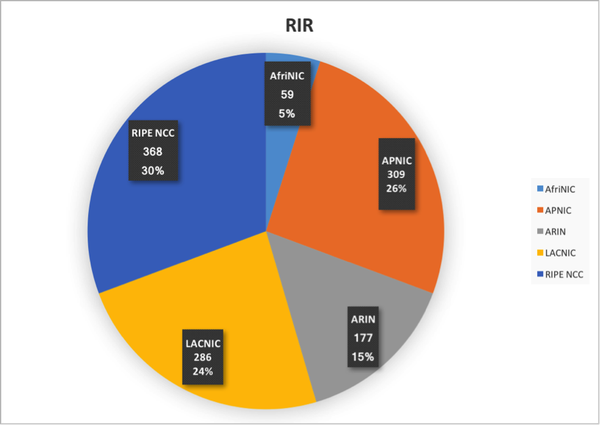
\includegraphics[width=\textwidth,height=\textheight,keepaspectratio]{survey2016_rir.png}
\caption{IPv6 survey 2016 RIR \autocite{Martinez2016}}
\end{figure}

Hoe gecommercialiseerd is IPv6 binnen de ISP’s nu? Wel, volgende grafiek geeft hierop een duidelijker beeld. Er wordt aangetoond dat 31\% van de ISP’s gebruik maken van IPv6 en commercieel actief mee bezig zijn. 17\% van de ISP’s is nog niet actief en dus ook nog niet commercieel actief, of zit momenteel in de test fase voor verdere stappen te ondernemen. De overige 52\% heeft deze vraag niet beantwoord. Daardoor kunnen we besluiten dat van alle deelnemers er 64\% van de ISP’s actief bezig is.

\begin{figure}
\centering
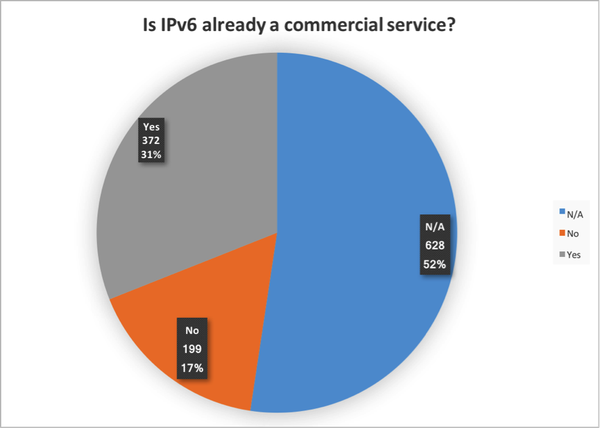
\includegraphics[width=\textwidth,height=\textheight,keepaspectratio]{survey2016_actief.png}
\caption{IPv6 survey 2016 commercieel \autocite{Martinez2016}}
\end{figure}

Op vlak van technologie is er veel keuze om klanten gebruik te laten maken van IPv6. Om een beter beeld te geven van de geprefereerde technologie keuzes van ISP’s is hieronder een grafiek die deze vraag beantwoord. Op het eerste zicht is er een groot deel dat gebruik maakt van FTTH, 35\%, xDSL, 22\%, en via kabel of DOCSIS, 20\%. 

\begin{figure}
\centering
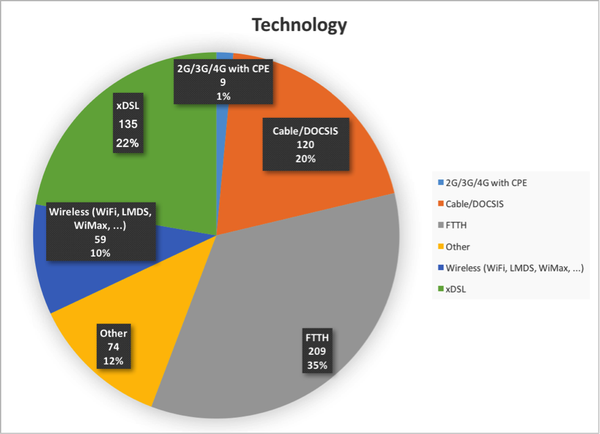
\includegraphics[width=\textwidth,height=\textheight,keepaspectratio]{survey2016_technologie.png}
\caption{IPv6 survey 2016 technologie \autocite{Martinez2016}}
\end{figure}

De laatste grafiek zal een verduidelijking weergeven op de gebruikte transitie mechanismen van een ISP. Bij transitie mechanisme zijn er veel verschillende methodes, maar welke het meest gebruikt worden onder de ISP’s is belangrijk om te weten. Op onderstaande grafiek is er een duidelijke winnaar. De methode die het meeste gehanteerd wordt is Dual-stack met een publiek IPv4 en Global unicast adres, GUA. In hoofdstuk 3 werd er dieper ingegaan op enkele methodes en uit de conclusie blijkt dat er een voorkeur was naar Dual-stack, wat hier ook bewezen is.

\begin{figure}
\centering
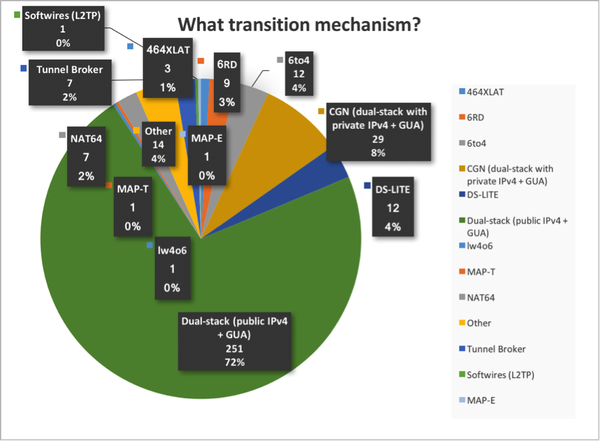
\includegraphics[width=\textwidth,height=\textheight,keepaspectratio]{survey2016_transitie.png}
\caption{IPv6 survey 2016 transitie \autocite{Martinez2016}}
\end{figure}

Om de evolutie op een jaar tijd te bekijken, gaan we deze resultaten vergelijken met de enquête die dateert van 13 oktober 2017. Met deze update is er een beter zicht mogelijk op de evolutie van IPv6 op een jaar tijd. Hierbij zullen de uitslagen vergeleken worden met de enquête van 2016. 

Opnieuw werd er gekeken hoever de commercialisatie stond van IPv6 bij ISP’s. Bij het opnieuw stellen van deze vraag is er een duidelijk verschil van resultaten ten opzichte van het vorige jaar.  Het grootste verschil is het aantal deelnemers die deze vraag niet beantwoord hadden. Bij de laatste update werd deze vraag volledig beantwoord en gaf dit een beter beeld van de effectieve commerciële diensten. Er waren maar liefst voor 65\%, 438 van de 673 deelnemers, van de antwoorden een ja-stem. Dit wil zeggen dat 65\% van de deelnemers actief bezig is met het aanbieden van IPv6 aan klanten. Waaronder het jaar ervoor maar 199 ISP’s bezig waren met het verdelen van IPv6.

\begin{figure}
\centering
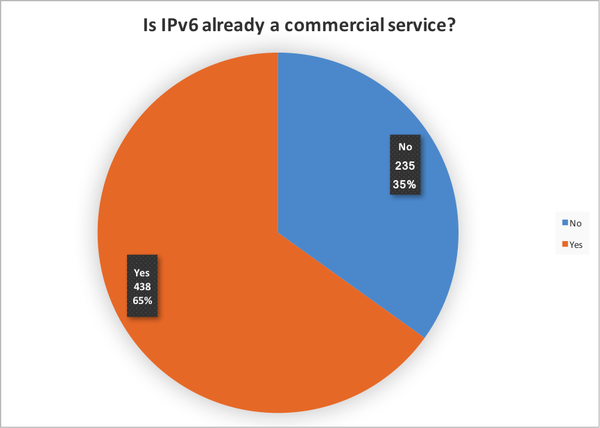
\includegraphics[width=\textwidth,height=\textheight,keepaspectratio]{survey2017_actief.png}
\caption{IPv6 survey 2017 commercieel \autocite{Martinez2017}}
\end{figure}

Op vlak van de gebruikte technologieën zijn er weinig veranderingen gebeurt op jaarbasis. De meest gehanteerde methodes blijven FTTH, xDSL en 3G broadband als bijkomende methode. Deze zijn voorlopig de meeste populaire technologieën. Hoewel in het jaar 2016 DOCSIS populair was, is deze verminderd naar gebruik toe.

Ook is er een overgang van gebruikte transitie mechanieken. Hierdoor blijkt dat nieuwere en recentere methodes worden gehanteerd in plaats van de oudere technieken. Het is zo dat er een groei is in het gebruik van 464XLAT en dual-stack met publieke IPv4 adressen. Verder is het zeker belangrijk om een nieuw evolutie-onderzoek op te stellen van het jaar 2017 tot 2018. Dit zou een nog beter zicht moeten geven over wat er echt aan het doorgroeien is naar een standaardoplossing voor dergelijke methodieken om met IPv6 te werken.

In 2018 werd er een interessante update van een bepaalde enquête uitgevoerd. Deze ging eerder over de adoptie wereldwijd en niet zozeer gefocust op ISP’s. Deze enquête werd uitgevoerd in verschillende jaren zoals 2008, 2009, 2011, 2012 en het laatste jaar 2013. Nu in 2018 werd er een update gemaakt voor de evolutie om de afgelopen 5 jaar te weerspiegelen en opnieuw informatie te verzamelen. RIPE heeft deze uitgevoerd en de eerste resultaten werden voorgesteld op het RIPE76 evenement in Marseille op 14-18 mei 2018. De uitgebreide resultaten zullen worden voorgesteld op 6 juni op het Educa evenement. Daarom zullen de eerste resultaten al onderzocht worden in deze scriptie.

In de verkregen resultaten is er te zien dat er ongeveer een 50\% van de antwoorden vooral uit grote ISP’s is gekomen, voor 30\% aan educatieve instellingen en ICT instellingen en voor 20\% aan overheid, onderzoekers en andere instellingen. Deze indelingen komen overeen met de jaren ervoor wat het zeer goed maakt omdat het over dezelfde aantal soorten instellingen gaat. Het probleem bij deze enquête was dat deze niet bereikbaar zijn vanaf IPv6. Waardoor er enkele resultaten wegvielen maar volgens RIPE was dit de bedoeling omdat deze hetzelfde moest opgesteld zijn als de jaren er voorheen.

Opvallende data die was geanalyseerd was de IPv6 allocatie. IPv6 allocatie betekent het toewijzen van adresruimte naar IR (Internet Registry) om op hun beurt terug die adresruimte door te verdelen. Momenteel staat het op 85\% IPv6 allocatie. Dit komt neer op een groei van 20\% met het jaar 2012 en een groei van 10\% met 2013. Het is logisch dat deze momenteel minder en minder zal groeien. Het is dus nog niet de bedoeling om 100\% al toe te wijzen en te verdelen.

\begin{figure}
\centering
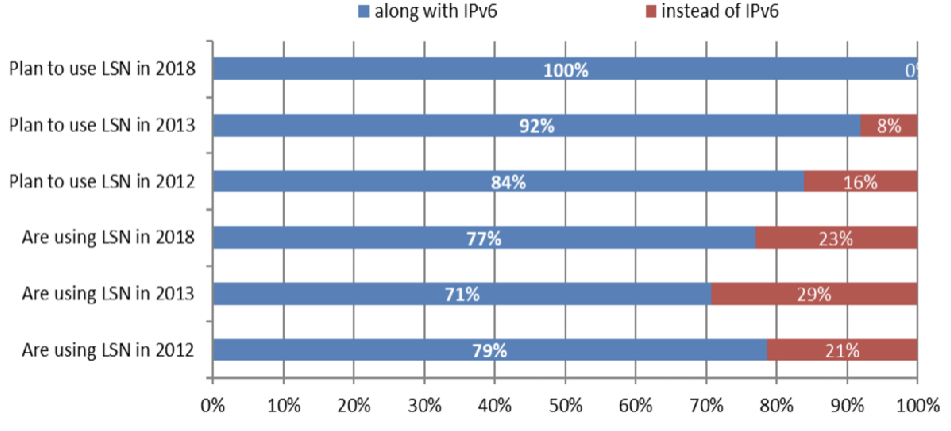
\includegraphics[width=\textwidth,height=\textheight,keepaspectratio]{survey2018_cgn.PNG}
\caption{IPv6 survey 2018 CGN/LSN \autocite{Massimiliano2018}}
\end{figure}

Alweer zijn de transitie technieken onderzocht en geanalyseerd naar welke het meeste aanvaard en gebruikt worden. Volgens deze data gebruikt meer dan 50\% geen transitie methode. Van diegene die wel deze technologie gebruiken kan er het volgende worden afgeleid. Op deze grafiek is er duidelijk te zien dat NAT64 een groot deel in beslag neemt en de populairste methode is. Daarnaast hebben DS-Lite en 6RD ook hun gebruikers maar bevatten deze een kleinere populariteit.

\begin{figure}
\centering
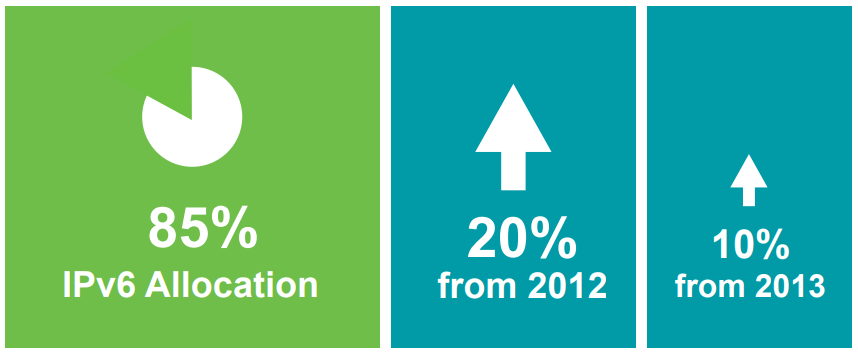
\includegraphics[width=\textwidth,height=\textheight,keepaspectratio]{survey2018_allocatie}
\caption{IPv6 survey 2018 verdeling \autocite{Massimiliano2018}}
\end{figure}

Ook is er iets interessant uitgehaald uit de verkregen data. Het gebruik maken van CGN (Carrier Grade NAT) of LSN (Large Scale NAT) samen of in plaats van IPv6. Met deze grafiek is er een zeer goed zicht op de toekomst van IPv6. In het jaar 2012 was er 16\% dat koos om deze technologie, CGN/LSN, te gebruiken in de plaats van IPv6. Het jaar daarop was dit met de helft verminderd en momenteel in 2018 staat het aantal geplande op 0\%. Dit is goed omdat men op deze manier gaat samenwerken met het IPv6 protocol en niet proberen deze te vervangen. Momenteel gebruiken er wel nog 23\% van deelnemers CGN/LSN als vervanger van IPv6. Als we dit vergelijken met het jaar 2013 zien we een kleine daling wat het overschakelen van vervangen naar samen met verbeterd. De komende jaren mogen we dus zeker verwachten dat deze enkel maar gaat afnemen omdat de geplande vervanging 0\% bevat.

\begin{figure}
\centering
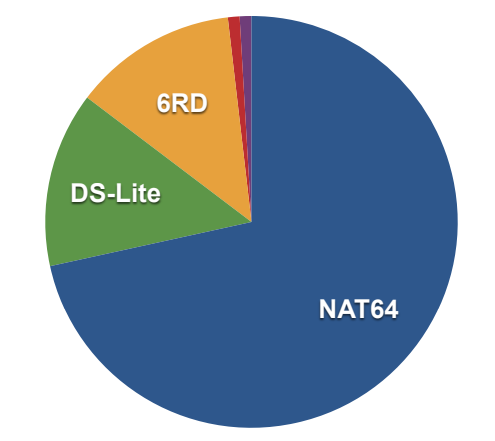
\includegraphics[width=\textwidth,height=\textheight,keepaspectratio]{survey2018_transitie.PNG}
\caption{IPv6 survey 2018 transitie \autocite{Massimiliano2018}}
\end{figure}

Nu we weten hoe het al gaat met IPv6, blijven er toch velen achter en durven ze vaak de stap niet te zetten naar IPv6. Daarom was er een bepaalde vraag gesteld om te achterhalen waarom het ondersteunen van IPv6 niet direct gebruikt wordt. Hier kwam er als duidelijk antwoord dat de kennis, bijkomende kosten en het overbrengen naar niet technische afdelingen het moeilijk maakt om dit te volbrengen. Als deze antwoorden werden vergeleken met de jaren voordien dan ziet men dezelfde antwoorden steeds terugkomen. Daarom blijft er vaak de vraag waarom er nog steeds geen verandering volgde en wat men daaraan kan doen.

In het volgende hoofdstuk zal er vooral dieper ingegaan worden op de adoptie in België en hoe deze daar aan het evolueren is. Aan de hand van grafieken zal er een duidelijk overzicht gegeven worden over de huidige aanpak van IPv6 op de Belgische markt.



